\PassOptionsToPackage{usenames,dvipsnames}{xcolor}
\documentclass[twocolumn,twocolappendix]{aastex63}

% Add your own macros here:
\pdfoutput=1 %for arXiv submission
%\usepackage{amsmath,amssymb,amstext}
\usepackage{amsmath,amstext}
\usepackage[T1]{fontenc}
\usepackage{apjfonts}
\usepackage{ae,aecompl}
\usepackage[utf8]{inputenc}
\usepackage[figure,figure*]{hypcap}

\usepackage{url}
\urlstyle{same}

\usepackage{lineno}
\linenumbers
%\modulolinenumbers[2]

\newcommand{\placeholder}[1]{\textit{PLACEHOLDER: #1}}

\newcommand{\EiffL}[1]{{\color{cyan}FL: #1}}
\newcommand{\denise}[1]{{\color{red}DL: #1}}

% header settings
\shorttitle{Differentiable Lensing Simulations}
\shortauthors{Lanzieri et al.\ (LSST~DESC)}

% ======================================================================

\begin{document}
\title{Forecasting the power of Higher Order Weak Lensing Statistics with automatically differentiable simulations}
\collaboration{1000}{The LSST Dark Energy Science Collaboration (LSST DESC)}
\noaffiliation

% paper leads
\author{Denise Lanzieri}
\affiliation{Université Paris Cité, Université Paris-Saclay, CEA, CNRS, AIM, F-91191, Gif-sur-Yvette, France}

\author[0000-0001-7956-0542]{Fran\c{c}ois Lanusse}
\affiliation{Université Paris-Saclay, Université Paris Cité, CEA, CNRS, AIM, 91191, Gif-sur-Yvette, France; }

%First Tier authors (alphabetical)
\author{Chirag Modi}
\affiliation{Center for Computational Astrophysics,
Center for Computational Mathematics,
Flatiron Institute, New York, NY 10010, USA}
% \noaffiliation

\author{Benjamin Horowitz}
\affiliation{Lawrence Berkeley National Laboratory, 1 Cyclotron Road, Berkeley, 94720, CA, USA}
\affiliation{Department of Astrophysical Sciences, Princeton University, Princeton, NJ 08544, USA}


\author{Joachim Harnois-Déraps}
\affiliation{School of Mathematics, Statistics and Physics, Newcastle University, Herschel Building, NE1 7RU Newcastle-upon-Tyne, UK}
% Second Tier authors (alphabetical)
\author{Jean-Luc Starck}
\affiliation{Université Paris-Saclay, Université Paris Cité, CEA, CNRS, AIM, 91191, Gif-sur-Yvette, France; }

\begin{abstract}
In this project we investigate the relative constraining power of various map-based higher order weak lensing statistics in an LSST setting. Such comparisons are typically very costly as they require a large number of simulations, and become intractable for more than 3 or 4 cosmological parameters. Instead we propose a new methodology based on the TensorFlow framework for automatic differentiation, and more specifically the public FlowPM N-body simulation code. By implementing ray-tracing in this framework, we will be able to simulate lensing lightcones, and compute Higher Order lensing statistics on the resulting maps. These statistics can then be differentiated with respect to cosmology, or any systematics included in the simulations, thus allowing, for exact Fisher forecasts.
\end{abstract}

\keywords{methods: statistical -- dark energy}

%\accepted{}
%\submitjournal{the Astrophysical Journal Supplement}


%\tableofcontents%-----------------------------
%===========================
% BEGINNING OF THE MAIN TEXT
%===========================

\section{Introduction}


\section{Methods}

%We compare the sensitivity of three different map-based statistics: angular power spectra, the peak counts and the $l_{1\text{norm}}$.
 %the calculation of the summary statistics, and the Fisher Forecast process. 


\subsection{{Weak lensing}}

Weak gravitational lensing is a promising observational technique to infer the projected matter density distribution between an observer and a source by measuring galaxy shape correlations. 
The effect of gravitational lensing 
can be quantified in term of the separation vector \textbf{x} between a ray and a fiducial ray separated by the angle $\boldsymbol{\theta}$ at the observer:
\begin{align}\label{sep}
   & \textbf{x}(\boldsymbol{\theta},\chi) =
    f_k(\chi)\boldsymbol{\theta} + \\
   &- \frac{2}{c^2}
    \int_0^{\chi}
    \text{d}\chi'
    f_k(\chi-\chi')
    [ \boldsymbol{\nabla_{\bot}}\Phi( \textbf{x}(\boldsymbol{\theta},\chi'),\chi')-
    \boldsymbol{\nabla_{\bot}}\Phi^{(0)}(\chi')
    ],
\end{align}
where we denote as $\Phi$ and $\Phi^{0}$ the potential along the two light rays, and as $f_k(\chi)$ and $\chi$ the angular and radial comoving distance.

The Jacobian matrix, describing the linearized lens mapping, is defined as:
\begin{equation}
\mathcal{A}(\boldsymbol{\theta},\chi)=
\frac{1}{f_{k}(\chi)}
\frac{\partial \textbf{x}}{\partial \boldsymbol{\theta}}.
\end{equation}
We know that the knowledge of the gravitational potential and the use of accurate solvers for light ray trajectories is computationally expensive. Nevertheless, the integral equation \ref{sep} can be approximated by considering the series expansion in power of $\Phi$ and truncating the series at the first term.
With this assumptions, and considering that $\nabla_{\bot}\boldsymbol{\Phi}^0$ does not depend from $\boldsymbol{\theta}$, the Jacobian matrix can be written as:
\begin{equation}
    \mathcal{A}_{ij}(\boldsymbol{\theta},\chi)
     =\delta_{ij}-\frac{2}{c^2}
    \int_0^{\chi} d\chi'
     \frac{f_k(\chi-\chi')f_k(\chi')}{f_k(\chi)}
     \Phi_{ij}(f_k(\chi')\boldsymbol{\theta},\chi').
\end{equation}
Notice that this approximation, also known as Born approximation, is only valid in the limit of weak-field metric (small $\Phi$). 


If we define the 2D potential, the \textit{lensing potential} as:
\begin{equation}
    \psi(\boldsymbol{\theta},\chi) \equiv
 -\frac{2}{c^2}
= \int_0^{\chi} d\chi'
   \frac{f_k(\chi-\chi')f_k(\chi')}{f_k(\chi)f_k(\chi')}
  \Phi(f_k(\chi')\boldsymbol{\theta},\chi').
\end{equation}
 the Jacobi matrix can be written as:
\begin{equation}
    \mathcal{A}_{ij}=\delta_{ij}-\partial_i \partial_j\psi. 
\end{equation}

From the parametrization of the symmetrical matrix $\mathcal{A}$, we can define the spin-two shear $\gamma=(\gamma_1,\gamma_2)$ and the scalar convergence field, $\kappa$. 
Hence, the convergence and the shear are defined as second derivative of the potential:
\begin{equation}\label{kshear}
    \kappa=\frac{1}{2}(\partial_1\partial_1+\partial_2\partial_2)\psi; \ \gamma_1=\frac{1}{2}(\partial_1\partial_1-\partial_2\partial_2)\psi; \ 
    \gamma_2=\partial_1\partial_2\psi;
\end{equation}

The two fields $\gamma$ and $\kappa$ describe the distortion in the shape of the image, and the change in the angular size, respectively.
By combining the 2D Poisson equation with the Eq.\ref{kshear} the convergence $\kappa$ becomes:
\begin{equation}
    \kappa_{born}(\boldsymbol{\theta})= \frac{3H_0^2 \Omega_m}{2c^2}
    \int_0^{\chi_s} 
    \frac{d\chi}{a(\chi)}
    g(\chi)
    \delta(f_k(\chi)\boldsymbol{\theta},\chi),
\end{equation}
where we define the \textit{lensing efficiency}
\begin{equation}
   g(\chi) \equiv
   \text{d}\chi'
   n(\chi')
    \frac{f_k(\chi'-\chi)}{f_k(\chi')}.
\end{equation}


Thus, the Born–approximated convergence can be interpreted as the integrated total matter density along the line of sight, weighted by the distance ratios and the normalised source galaxy  distribution $n(\chi)$d$\chi=n(z)$d$z$.


\subsection{Simulation}
It's well known that an common feature of statics beyond second-order is the absence of analytical models with which to predict the observed signals. Hence, we need to adopt a forward modelling approach and create a suite of numerical simulations. 
In the following section we introduce the mass map simulation procedure, including a description of the simulator and of the construction of the weak lensing lightcone.

\subsubsection{FLOWPM}
Our weak lensing simulation tool is based on FlowPM (/cite Modi, Lanusse et al. ), a fast particle-mesh solver that implements the time integration for gravitational evolution starting from the Gaussian initial conditions of the Universe to the observed large scale structures through a Kick-Drift scheme.


After instantiating the $\Lambda$CDM cosmology with our desired parameters, (the initial power spectrum and the evolution of the particles depend from $\sigma_8$ and $\Omega_{c}$) we created the initial condition for the N-body simulation using the normalised linear matter power spectrum as implemented by (/cite Eisenstein and Hu of '98 ) and generated the linear field at requested scale. After that, we implemented the N-body. As said before, The N-body simulation does the time integration of a given initial linear field  across a given array of scale factors implementing a series of Kick-Drift-Kick operations. 
During the \textit{Kick} operation we estimate the gravitational force experienced by every particles implementing Fast Fourier Transform and update their momentum. In the next state, \textit{Drift}, the particles are displaced and their positions is updated with the velocity estimated in the previous step. This operation is continued until the observed large scale structures at the final time-step.
To perform the lightcone computation and extract the lens planes,  we export several intermediate state from the N-body simulation. From a given intermediate state we extract a slice and project it as a density plane by painting the particles on a 2D mesh. 
After creating a grid of coordinates, the lens planes are interpolated onto sky coordinates. 
 At this point, we have constructed a ray tracer object, to compute the convergence, we directly integrate the lensing density along the unperturbed line of sight. 

    
\subsubsection{Additional validation for our ray-tracing implementation } 
As an additional test to validate our ray-tracing, instead of running the N-body simulation to generate the snapshots of particles for different scale factors, we create these snapshots by using a linear matter power spectrum at a given fixed redshift $z=0.52$ . \\
Specifically, we estimate the initial LPT displacement given an input linear (real) field.

As we said, the aim of this test is to prove the validity of our ray-tracing. In principle, without the N-body simulations and his possible approximations and systematics, any disagreement between the angular power spectrum computed from the final convergence map
and the angular power spectrum we use as reference can be attributable to the ray-tracing.

Fig. shows a comparison between the theoretical linear matter power spectrum computed using the Jax-cosmo library at the redshift $0.52$ and the matter power spectrum computed from the resulting snapshots, after applying the painting operations. As we can see the matter power spectrum start to lack in power for $k$(maggiore o circa uguale)1. This is probably due to the paint operation and is something to take into account when we will study the final power spectrum.



From the full projected boxes of the simulations, we exported the lens planes, then interpolated on the light-cones. 


The final angular power spectrum is obtained averaging over 1000 samples.


\subsubsection{Potential Gradient Descendent (PGD)}    
Fast N-body simulations can be used as viable alternative to full N-body to model the galaxy statistics and create fast and low computational costs realizations of the large scale structures. Nevertheless, this kind of simulations lack resolution on small scale and can't give accurate halo matter profiles or matter power spectrum. 


To recover this missing accuracy, we employs the PGD scheme (\cite{Dai_2018}). 
The main goal is to mimic the physics lost in the low resolution simulations by computing the short range force operation as an additional correction displacements in a post-processing step. \\
The additional displacement is computed by pointing the particles towards a filtered potential minimum of the particle mesh solver.


%\begin{equation}\label{displacement}
 %   \textbf{S}=4\pi G \bar{\rho}\alpha_{PM}/H_0^2 \nabla(
  % \hat{\textbf{O}}_l(k)
   %  \hat{\textbf{O}}_s(k)
    %\nabla^{-2}\delta),
%\end{equation}
%where $\hat{\textbf{O}}_l(k)= \exp{(\frac{k^2}{k^4_l})}$ and $\hat{\textbf{O}}_s(k)= \exp{(-\frac{k^4}{k^4_s}})$ are the low and high pass filter introduced to remove the long range force and to reduce the numerical effect induced by the mesh resolution. \\
PGD introduces control parameters that can be tuned by comparing the matter power spectrum to a reference power spectrum. 


We employ an online-PGD technique worth mentioning here: the correction involved in computing additional displacements is computed after every drift step in the N-body simulation. 


We find that a PGD correction computed directly at the end of the simulation fails, introducing some significant sharp clusters or changing the shape of some of the structures. Effectively this is equivalent to requesting a too large correction at once, which our method avoids.

In practice we set it up so that it takes the power spectra at all intermediate redshift and fits the PGD parameters as to recover the \textit{Halofit} non linear power spectrum.



Figure \ref{fig:pkhalofit_comp} shows the matter power spectrum at $z=1.69$ of our simulations before and after applying the PGD correction compared to analytic Halofit predictions (\denise{cita}(Smith et al. 2003; Takahashi et al. 2012)).
\begin{figure}
    \centering
    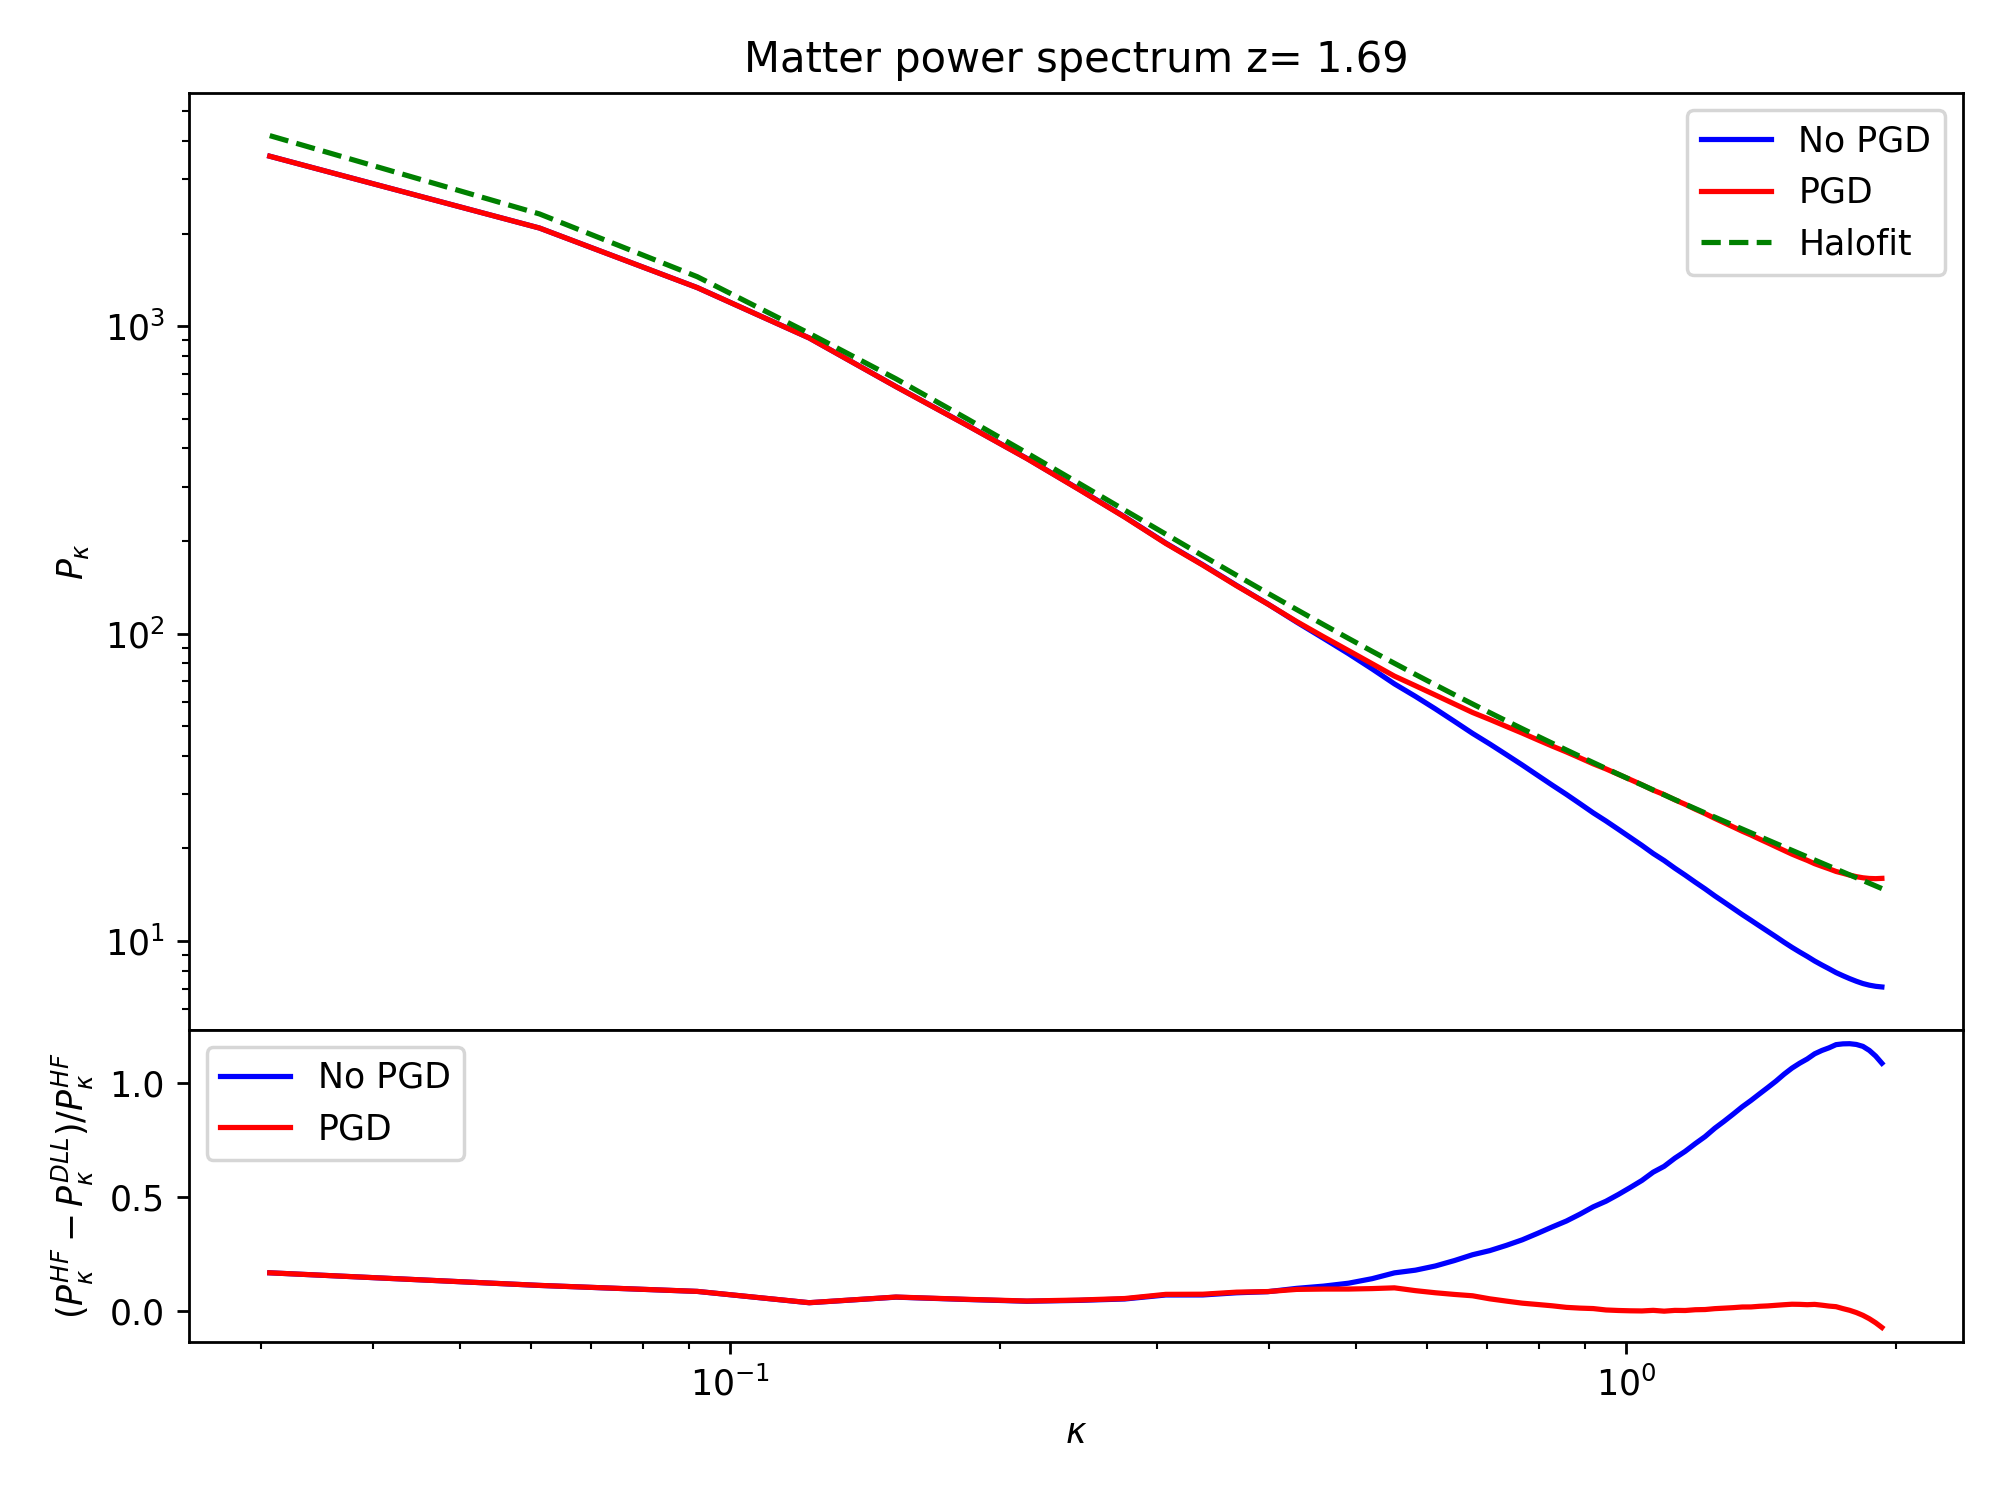
\includegraphics[width=\columnwidth]{paper/figures/pkhalofit_comp.png}
    \caption{
    Upper panel: Comparison of the matter power spectrum of FlowPM before and after the PGD correction with reference matter power spectrum \textit{Halofit} at redshift $z = 1.69$. Lower panel: Fractional differences between FlowPM and Halofit.
    }
    \label{fig:pkhalofit_comp}
\end{figure}

In Figure \ref{fig:comp_kmap} we show an example of our convergence map at $ z= 1.034$, as well as the same map when the PGD correction is not applied. 
We can see that the structures are not modified but simply sharpened.
\begin{figure*}
    \centering
    \includegraphics[width=0.9\textwidth]{paper/figures/kmap_compgd.png}
    \caption{ \textbf{Left panel}: An example of our convergence map at source redshift $z= 1.034$.
    \textbf{Right panel}: Same convergence map when the PGD correction is not applied.}
    \label{fig:comp_kmap}
\end{figure*}

In Figure \ref{fig:ps_comp} in the upper panel, we present the DLL angular power spectrum complemented by the PGD scheme to a conventional DLL simulation with the same resolution. Both the outputs are compared to the analytic Halofit prediction for the angular power spectrum. In the lower panel the fractional differences between the our maps and the analytic Halofit prediction.  Both the power spectra and ratios are averaged over $N = 100$ realisations.
We can conclude that PGD scheme allows to achieve higher accuracy at the same computational cost.
 


\begin{figure}
    \centering
    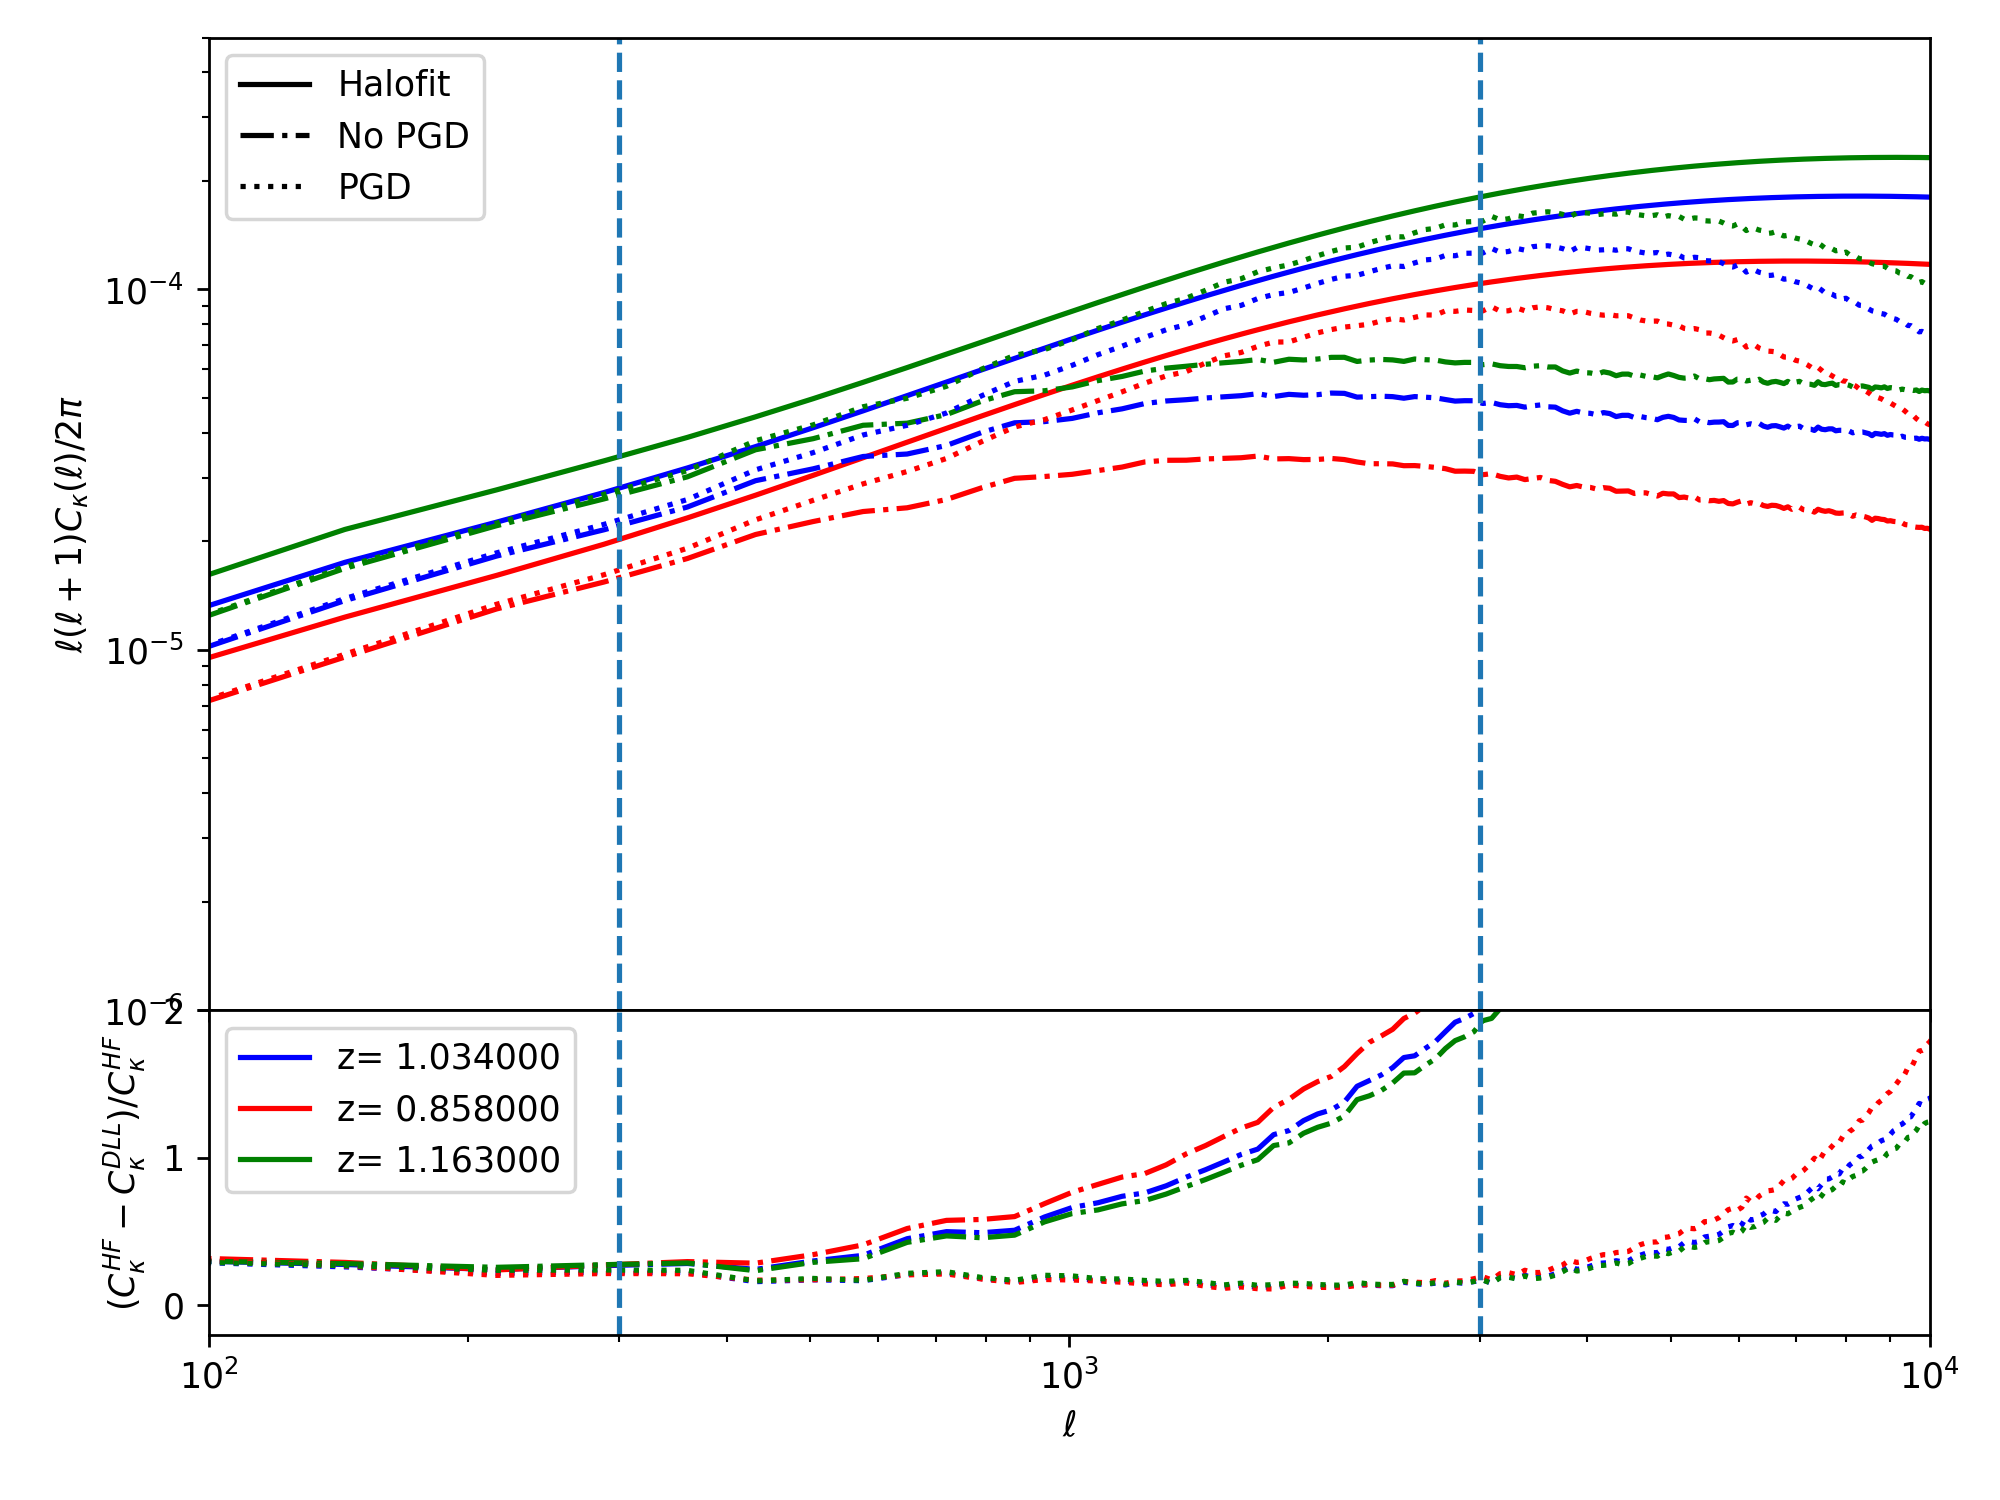
\includegraphics[width=\columnwidth]{paper/figures/clshalofit_comp.png}
    \caption{
    \textbf{Upper panel}: Angular power spectra for 3 different source redshifts from
our DLL maps. \textbf{Lower panel}: Fractional differences between the
DLL and Halofit power spectra for 3 source redshifts. The power spectra and ratios are means over 100 map realisations. The two vertical lines define the range of $\ell$ between $[300,3000]$.}
    \label{fig:ps_comp}
\end{figure}



\subsection{Summary statistics}
In this work, in order to extract the cosmological information from the simulated $\kappa-$maps, we use tree summary statistic for weak lensing observable: the angular power spectrum, the `starlet peak counts' and the `starlet $l_{1\text{norm}}$'. 

We reproduce the analysis choices of the LSST Y1 data. The DESC science requirements document can be found here \cite{mandelbaum2018lsst}.
In particular we use a $n_{\text{eff}}=10$ galaxies per $\text{arcmin}^2$ for lensing sources and a $\sigma_e=0.26$ per component.


\subsubsection{Lensing Angular Power Spectrum}
Second order statistics, both in the form of shear 2-point correlation function $\xi_{\pm}(\theta)$, or its counterpart in Fourier space, the angular power spectrum $C_{\ell}$, have been widely used to extract the cosmological information from weak lensing mass maps. \
In the Limber approximation, the angular power spectrum of the convergence field can be computed as:
\begin{equation}
    C_{\kappa}(\ell)=\frac{9\Omega_m^2H_0^4}{4c^4}
    \int_0^{\chi_{lim}} \text{d}\chi 
    \frac{g^2(\chi)}{a^2(\chi)}P_{\delta}
    	\left( k=\frac{\ell}{f_K(\chi)},\chi \right),
\end{equation}
where $P_{\delta}$ defines the matter power spectrum of the density contrast.

In this paper, the angular power spectrum is computed from the noisy smoothed convergence maps: to each mock $\kappa$map we add Gaussian noise and than convolved it with a Gaussian smoothing kernel.


To understand how accurate our simulations are, and to validate the choice of the smoothing size to apply, we tried to reproduce the summary statistics from the only Dark $\kappa-TNG$ simulations. 
 We show the results from the angular power spectrum comparison for 3 source redshifts in Figure \ref{fig:ps_comp}.
\begin{figure}
    \centering
    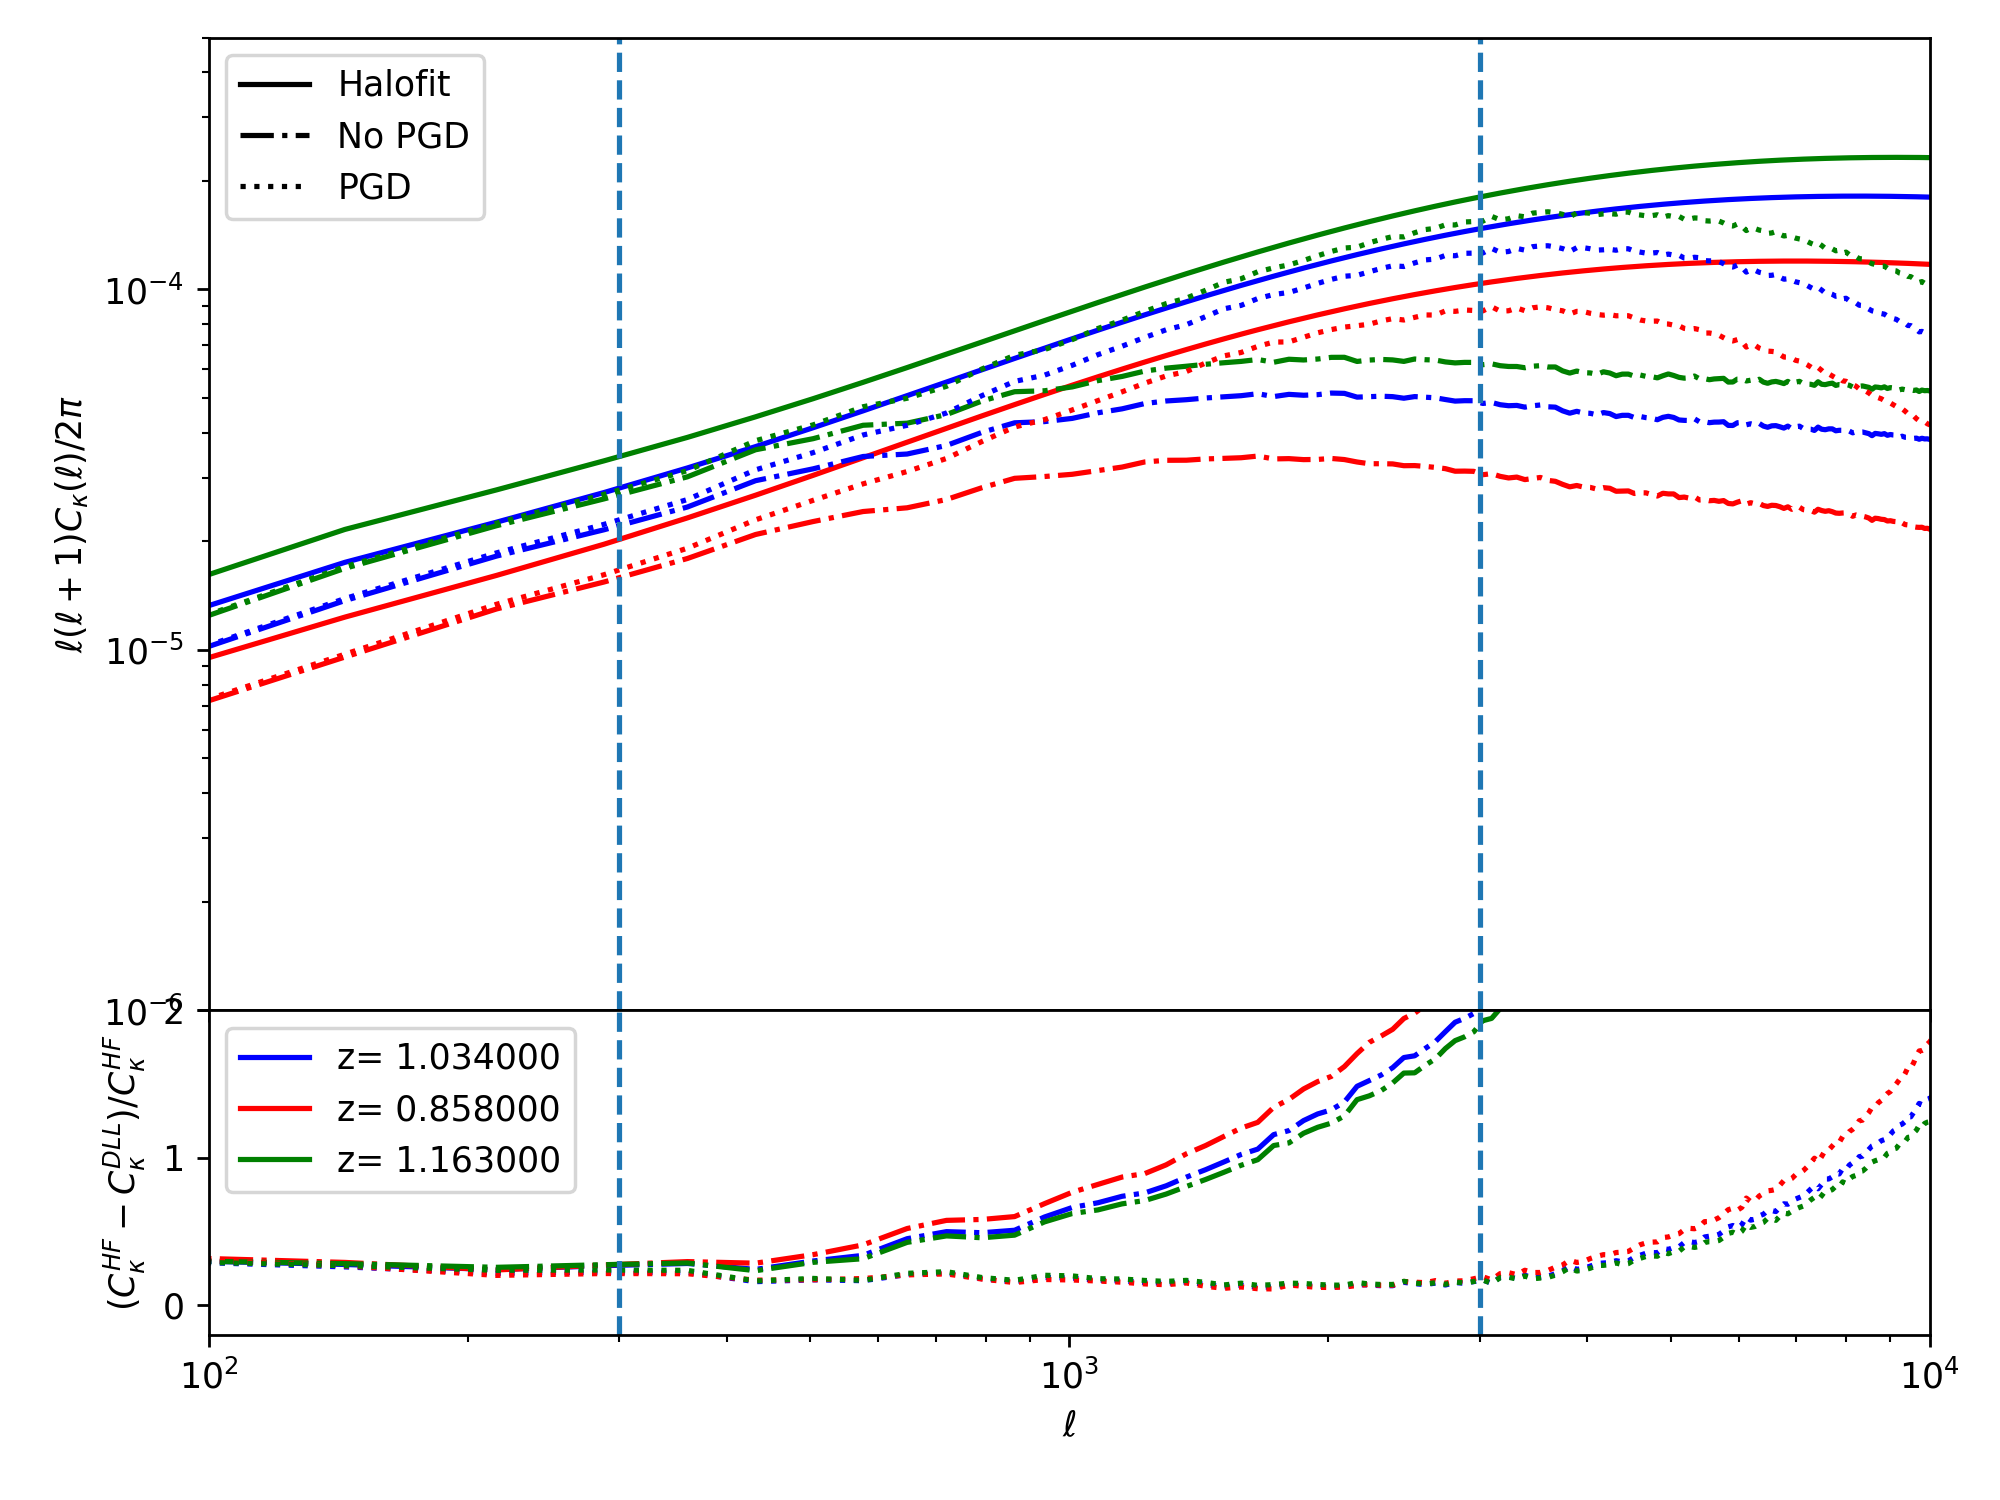
\includegraphics[width=\columnwidth]{paper/figures/clshalofit_comp.png}
    \caption{
    \textbf{Upper panel}: Angular power spectra for 3 different source redshifts from
our DLL maps. \textbf{Lower panel}: Fractional differences between the
DLL and Halofit power spectra for 3 source redshifts. The power spectra and ratios are means over 100 map realisations. The two vertical lines define the range of $\ell$ between $[300,3000]$.}
    \label{fig:ps_comp}
\end{figure}
% with a smoothing size $\theta=3.6$. We perform the angular power spectrum analysis in a range of $\ell=[300,3000]$ according to the requirement specified in  \cite{mandelbaum2018lsst}. 

For each map, we compute the power spectrum by using our own code implemented in the Tensorflow framework and we take the average over 2000 maps realisation.

\subsubsection{Wavelet Peak Counts}
It has been shown that it's necessary to go beyond second-order statistics to fully capture the non-Gaussian information encoded in the peak of the matter distribution. Several studies have proved that the  weak-lensing peak counts provide a way to capture information from non-linear structures that it is complementary to the information extracted by power spectrum.
The peak counts identify region of weak lensing map where the density value is higher, in this way they rely to the massive structure.
There are different ways to record the weak lensing peaks: the number of peaks as a function of either the signal-to-noise ratio or the convergence $\kappa$ of the peaks. 
In this paper, we choose to bin the peaks as function of $\kappa$. 
As for the angular power spectrum, the weak lensing peaks are detected from the noise and smoothed simulated maps by using our own code and by averaging over 2000 different realizations. A peak is identified as the pixel of larger value than its eight neighbors in the image, convolved with a starlet filter $\mathcal{W}(\theta_{\text{ker}})$:
\begin{equation}
    \textbf{Peaks}=(\kappa*\mathcal{W})(\theta_{\text{ker}})
\end{equation}
 We consider the peak distribution for 8 linearly spaced bins within the range $\kappa=[-0.05, 0.05]$. The bins are chosen such that at least 30 peaks are recorded in each bin. 

\EiffL{Explain wavelets}

One of the difficulties with traditional peak counting is that it relies on building
an histogram of peak intensities, and histograms, due to the discrete nature of the bins, are not differentiable. However, the underlying idea of peak counting is just to build an estimate of the density distribution of number of peaks as a function of their intensity. Histograms are one way to build such an estimate, and have been historically preferred, but for no particular reason. To circumvent the non-differentiability of histograms, we prefer here to estimate this density using an alternative method: Kernel Density Estimation (KDE). As a continuous equivalent to an histogram, KDEs are differentiables and can just as well be used to define the peak counts statistic.

\subsubsection{Wavelet $\ell_1-$norm}




\EiffL{Explain what's the deal with this l1 norm}

\section{Systematic effects}
Many systematic effects can influence the outcome of cosmic shear analysis and bias cosmic shear results. 
In this work we incorporate a treatment of the galaxy intrinsic alignment and photometric redshift uncertainty.
In the following, we introduce an overview of these systematics and outline how we incorporate in our analysis.

\subsection{Photometric redshift uncertainty}
Cosmic shear measurement require a large number of images, for such quantities, determining the redshift of the galaxies spectroscopically is not possible, for this reason, photometric redshift (''photo-z'') measurement are computed.
In this paper we use the Fisher formalism to investigate its impact on cosmological parameter estimation.
For our analysis we considered a Smail-type galaxy distribution p(z) (Smail et al. 1994),
\begin{equation}\label{photz}
    p(z) \propto z^{\alpha} e^{-(\frac{z}{z_0})^{\beta}}
\end{equation}

 We adopt  $\alpha=$, $\beta =$ and fix $z_0$ such that ?'

 We take into account the uncertainty of the redshift distributions by introducing  a shift of the distributions defined by Eq.\ref{photz} according to the nuisance parameters $\Delta_z$:
 \begin{equation}
     n'_i(z)= n_i(z-\Delta_z)
 \end{equation}

\subsection{Galaxy intrinsic alignment}

The galaxy ellipticity observed by a telescope is the combination of the cosmic shear signal $\gamma$ and the intrinsic shape of the source $\epsilon_{int}$, the latter can be further decomposed into the alignment term $\epsilon_{IA}$ and the random component $\epsilon_{ran}$. 

Several theoretical models have been proposed to described the physics of IA, such as the Non-Linear tidal Alignment model (e.g. in Bridle et King 2007), the tidal torquing model (described in Hirata et Seljak 2004; Catelan et al. 2001), or the combination of both (the Tidal Alignment and Tidal Torquing model, see Blazek et al. 2019).

The NLA model describes the IA as a linear coupling between the intrinsic galaxy shapes and the non-linear large projected tidal fields, the "non-linear" definition arises from the use of the non linear matter power spectrum in the computation. 

The IA signal can be decomposed into two components: 1) the intrinsic-intrinsic (II) term, describing the correlation of intrinsic ellipticities of two galaxies $i$ and $j$ and 2) intrinsic-shear coupling (GI) term, describing the correlation between the intrinsic ellipticity of one galaxy with the shear of another galaxy (\cite{kilbinger2015cosmology}).

The first step to introduce the IA term in our simulation, consists in computing the projected tidal field from the three-dimensional mass over-density field $\delta(\vec{x}$
as (\cite{harnois2021cosmic})
\begin{equation}
   \tilde{s}_{ij,2D}(\textbf{k}_{\bot})=
   2 \pi 	\left [ \frac{k_ik_j}{k^2}- \frac{1}{3} \right ]
   \tilde{\delta}_{2D}(\textbf{k}_{\bot})
   \mathcal{G}_{2D}(\sigma_g)
\end{equation}
where $\sigma_g$ is the smoothing scale of a two-dimensional smoothing kernel $\mathcal{G}_{2D}$, the tilde symbols $~$ refers to the Fourier transformed quantities, $\textbf{k}_{\bot}$ denotes the two Fourier wave-vector components perpendicular to the line of sight, and the indices $(i,j)$ represent the $x$ or $y$ component.
In this work we use a Gaussian kernel and set the values of $\sigma_g=(idk yet) h^{-1}$Mpc.
First of all, we computed the Fourier transform of the projected density field from the full boxes of the simulation. 
Then the smoothed tidal field is interpolated on the light-cone. 
Then, we couple the tidal field $s_{ij,2D}$ with the complex intrinsic ellipticities as (\cite{harnois2021cosmic}):
\begin{equation}
    \epsilon_{1}^{IA}=\frac{A_{IA\bar{C}_1\bar{\rho}(z)}}{D{z}} (s_{xx}-s_{yy}), \ \ 
      \epsilon_{2}^{IA}=-\frac{2A_{IA\bar{C}_1\bar{\rho}(z)}}{D{z}} s_{xy},
\end{equation}
(\denise{check this formula})
and compute the observed ellipticities as:
\begin{equation}
    \boldsymbol{\epsilon}^{obs}=
    \frac{\boldsymbol{\epsilon}^{int}+\textbf{g}}{1+\boldsymbol{\epsilon}^{int,*}\textbf{g}}, \ \  \text{with}  \ \
    \boldsymbol{\epsilon}^{int}=
    \frac{\boldsymbol{\epsilon}^{
     IA}+\boldsymbol{\epsilon^{ran}}}
     {1+\boldsymbol{\epsilon}^{IA,*}\boldsymbol{\epsilon^{ran}}}.
\end{equation}



 


\begin{figure}
    \centering
    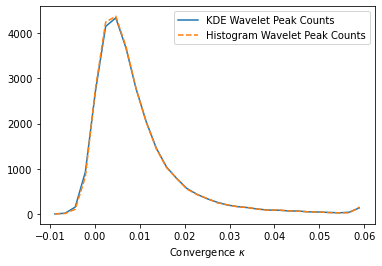
\includegraphics[width=\columnwidth]{figures/peakcounts.png}
    \caption{Comparison of traditional histogram-based peak counts, against our  KDE-based peak counts statistic. The two statistics are similar, but our KDE-based statistics is differentiable.}
    \label{fig:comp_statistics}
\end{figure}

\section{Fisher Forecast}
Fisher forecast is a widely used tool in cosmology for different purposes, e.g. investigate the impact of systematic sources. It can be thought as a tool to forecast error from a given experimental set up e quantify how much information we can extract from it. 

Compared to other methods, such as the Markov chain Monte Carlo method, is extremely fast, however, several issues have to be taken into account. 
The Fisher matrix is defined as the expectation value of the Hessian matrix of the likelihood $\mathcal{L}(C(\ell);\theta)$:
\begin{equation}
    F_{\alpha \beta}=\left \langle 
    \frac{\partial^2\mathcal{L}}
    {\partial \theta_{\alpha}\partial \theta_{\beta}}
    \right \rangle .
\end{equation}

where we indicate with $\theta$ the cosmological parameters or any systematics included in the simulation.
If we assume a Gaussian likelihood and a Covariance matrix $C_{ij}$ independent from $\theta$, we can calculate the Fisher matrix as
\begin{equation}\label{Fisher_matrix}
      F_{\alpha \beta}= \sum_{ij}\frac{\partial \mu}{\partial \theta_{\alpha}} C_{ij}^{-1}
      \frac{\partial \mu}{\partial \theta_{\beta}}
\end{equation}
were we indicate as $ \frac{\partial \mu}{\partial \theta_{\alpha}} $ the derivatives of the summary statistics evaluated at the fiducial parameter values.
In this paper, to compute the covariance matrix $C_{ij}$, we use 2000 independent simulations at the fiducial cosmology. 
We assume a parameter-independent covariance matrix computed as:
\begin{equation}
    C_{ij}=\sum_{r=1}^N
    \frac{(x_i^r-\mu_i)(x_i^r-\mu_)}{N-1}
\end{equation}
where $N$ is the number of independent realizations and $x_i^r$ is the value of the summary statistics in the $i^{th}$ bin for a given realization $r$ and $\mu$ is the mean of the summary statistics over all the realization in a given bin. 
Furthermore, we scale the covariance matrix by the ratio $f_{\text{map}}/f_{\text{survey}}$, where $f_{\text{map}}$ is the angular extend of our $\kappa$map and $f_{\text{survey}}$ is the étendue of the \textit{Vera C. Rubin Observatory}.
The derivatives of the summary statistics in the Eq.\ref{Fisher_matrix} are computed averaging over 250 independent fiducial simulations.


\section{Results}

\section{Discussion}

\subsection{Future directions}

\section{Conclusions}

%=====================
% END OF THE MAIN TEXT
%=====================


%%%%%%%%%%%%%%%%%%%% REFERENCES %%%%%%%%%%%%%%%%%%

\bibliography{biblio.bib}

%%%%%%%%%%%%%%%%%%%%%%%%%%%%%%%%%%%%%%%%%%%%%%%%%%
\end{document}
